% !TEX encoding = UTF-8
% !TEX TS-program = pdflatex
% !TEX root = ../tesi.tex

%**************************************************************
\chapter{Tecnologie e strumenti}
\label{cap:tecnologie_e_strumenti}
%**************************************************************
In questo capitolo verranno illustrate le tecnologie e gli strumenti che sono stati utilizzati per realizzare il progetto di stage.\\
Il capitolo si apre con una descrizione di che cos'è una \textit{Blockchain} e del perchè è stata scelta come tecnologia chiave per la realizzazione del progetto e, di seguito, verranno descritti tutti gli strumenti utilizzati.\\\\
Questa sezione è frutto di studi di vari documenti e \textit{whitepaper} forniti dall'azienda\cite{spidchain_whitepaper}\cite{SSID}\cite{jolocom_whitepaper}\cite{ITF_gartner}\cite{hashgraph_whitepaper}
%**************************************************************
\section{Cos'è una Blockchain}
Una \textit{Blockchain} è un \emph{\gls{dlt}}\glsfirstoccur che si basa fortemente sul \textit{consenso} e su un sistema di \textit{smart contracts}.
È quindi una piattaforma costruita su una rete di nodi (detti blocchi) distribuiti dove gli elementi chiave che la contraddistinguono sono:
\begin{itemize}
	\item \textbf{Smart Contracts} - programmi che vengono eseguiti solamente quando si verificano determinate condizioni;
	\item \textbf{Consenso} - sistema che assicura che la maggioranza (50\% + 1) dei nodi della rete identifichi e sia in accordo, con tutti gli altri nodi della rete, che un determinato stato del sistema sia quello esatto.
\end{itemize}
Questi blocchi sono formati da quattro sezioni:
\begin{itemize}
	\item \textbf{Block size} che rappresenta la grandezza in bytes del blocco;
	\item \textbf{Block Header} è un campo particolare che è a sua volta formato da:
	\begin{itemize}
		\item \textbf{Version} numero di versione del software utilizzato;
		\item \textbf{Previous Block Hash} contiene l'hash dell'header del blocco precedente.;
		\item \textbf{Markle root} hash della radice del \textit{Markle tree} (spiegato di seguito);
		\item \textbf{Timestamp} tempo di creazione del blocco;
		\item \textbf{Difficulty target} numero che indica il livello di difficolta per l'aggiunta del blocco alla \textit{Blockchain};
		\item \textbf{numero casuale o pseudo-casuale dato come risultato dell'elaborazione della \emph{\gls{pow}}\glsfirstoccur}.
	\end{itemize}
	\item \textbf{Transaction counter} contiene il numero di transazioni che compongono il blocco;
	\item \textbf{Transaction} lista di tutte le transazioni che verranno processate nel blocco.
\end{itemize}
\subsection{Caratteristiche chiave}
Abbiamo spiegato,a grandi linee, che cos'è una \textit{Blockchain} ma perchè questa dovrebbe essere una buona candidata per la realizzazione del modulo \gls{ITF}?\\
La risposta sta in tre caratteristiche che sono parte integrante del concetto stesso di \textit{Blockchain} e che la rendono un'ottima struttura anti-manomissione:
\begin{itemize}
	\item Funzione crittografica di hash;
	\item Strutture dati con hash pointer;
	\item Protocollo di consenso distributio.
\end{itemize}
Le funzioni \textit{crittografiche di hash}, unite agli \textit{hash pointer} fanno sì che la struttura dati complessiva sia immutabile il che è la base del'anti-manomissione della \textit{Blockchain}.
Se un utente malevolo modifica un dato in uno qualsiasi dei blocchi della \textit{Blockchain} questo farà sì che il puntatore hash the blocco successivo sia incorretto. Questo permette oltre di individuare un tentativo di manomissione anche di capire quale blocco è stato manomesso.\\
Per comprendere meglio questi concetti vediamo nel dettaglio le tre caratteristiche.
\subsubsection{Funzione crittografica di hash}
È una funzione matematica che converte un input di qualsiasi grandezza in un output di grandezza fissa.\\
Le funzioni crittografiche di hash hanno due proprietà fondamentali:
\begin{itemize}
	\item \textbf{Collision-resistant} - è difficile, quasi impossibile, che due input diversi creino lo stesso output;
	\item \textbf{Enabke hiding} - non è possibile, partendo dall'output, recuperare l'input iniziale.
\end{itemize}
Un esempio di algoritmo che rispetta queste caratteristiche è \emph{\gls{sha256}}\glsfirstoccur.

\subsubsection{Strutture dati con hash pointer}
Gli \textit{Hash pointer} sono particolari strutture dati che contengono:
\begin{itemize}
	\item un puntatore a dove sono immagazzinati i dati;
	\item l'\textit{hash} crittografico dei dati alla quale il puntatore fa riferimento
\end{itemize}
Questo fa sì che sia possibile, oltre che recuperare le informazioni, verificare, tramite l'\textit{hash}, che le informazioni recuperate siano corrette e non manomese.\\
Grazie a questa tipologia di struttura dati, la \textit{Blockchain} realizza un altra struttura di fondamentale importanza per il funzionamento del sistema il \textit{Markle Tree}.\\
Questa tipologia di struttura non è altro che un albero binario che, tramite l'ausilio degli \textit{hash pointer}, mantiene al suo interno i dati e le transazioni di ogni blocco che fa parte della \textit{Blockchain}.\\
I dati, contenuti nelle foglie dell'albero, vengono crittografati tramite \textit{hash} e posti su un nodo padre di livello superiore. Qui, i nodi padre, vengono raggruppati a coppie, calcolato il loro \textit{hash} e posti a loro volta in un livello superiore. 
Continuando a raggruppare i nodi padre e facendo l'\textit{hash} si arriva fino all'apice dell'albero che va a formare il \textit{Markle tree root.}
Se qualcuno prova a manomettere uno qualsiasi dei blocchi di dati sottostanti farà sì che l'\textit{hash pointer} ai livelli più alti non corrisponda più a quello calcolato.
\begin{figure}[!h]
	\centering
	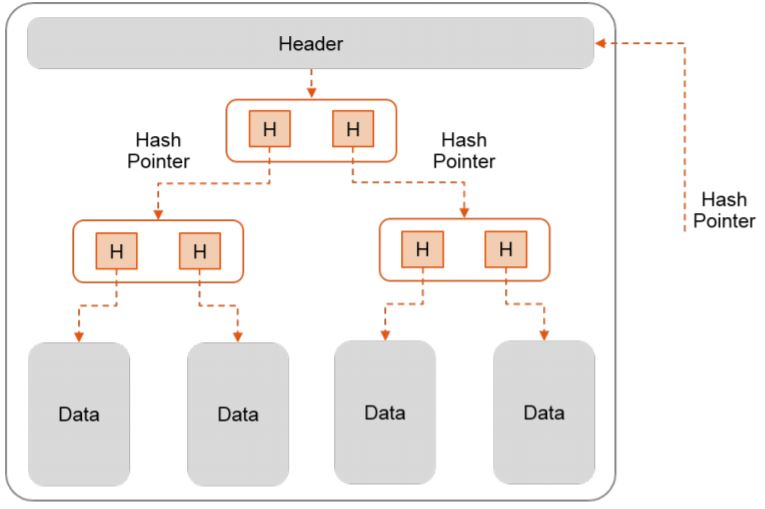
\includegraphics[scale=0.50]{immagini/markle_tree}
	\caption{Rappresentazione di un Markle Tree}
\end{figure} 
\subsubsection{Protocollo di consenso distribuito}
Uno dei punti di forza della \textit{Blockchain} è la decentralizzazione del sistema che crea. Per questo motivo è di fondamentale importanza avere un \textit{protocollo di consenso distribuito} che fa sì che ogni nodo partecipante nella rete sia d'accordo su cosa deve essere scritto nella \textit{Blockchain}.
L'algoritmo di consenso assicura due proprietà, sotto la condizione che tutti i nodi abbiamo ricevuto qualche forma di informazione:
\begin{enumerate}
	\item L'algoritmo termina quando tutti i nodi "onesti" (non malevoli e quindi nodi che non vogliono introdurre informazioni errate all'interno della rete) concordano (accettare l'informazione e scriverla sulla Blockchain o rifiutarla) sull'informazione ricevuta;
	\item L'algoritmo assicura che l'informazione sia generata da un nodo "onesto".
\end{enumerate}
In questo caso, un nodo "onesto" viene scelto per "agganciare" il nuovo blocco, contenente i nuovi dati ricevuti, alla \textit{Blockchain} e gli altri nodi replicano il cambiamento di stato sulla propria rete \textit{Blockchain}. In questo modo si riesce a generare fiducia tra tutti i nodi quando, tra di loro, non si conoscono e non si fidano.

\subsection{Tipologie di Blockchain}
La rete \textit{Blockchain} è disponibile in due versioni differenti:
\begin{itemize}
	\item \textbf{Permissionless Blockchain} - è detta anche \textit{Blockchain pubblica} perché tutti possono partecipare alla rete. Non vi è alcun tipo di controllo che governa la partecipazione alla rete o che ne limiti l'accesso.  Il comportamento dell'interno sistema è tutto in mano al protocollo di consenso distribuito;
	\item \textbf{Permissioned Blockchain} - è detta anche \textit{Blockchain privata} perché per poter avere accesso alla rete e potervi quindi partecipare è necessaria la verifica da parte di nodi già interni alla rete che autorizzino o meno l'accesso a nuovi nodi.
\end{itemize}
La scelta tra \textit{permissioned} o \textit{permissionless} è guidata principalmente dal tipo di applicazione o servizio che si vuole sviluppare o fornire e dalla necessità o meno di avere controllo su chi può partecipare alla rete.
Per l'implementazione di un \gls{ITF} sono necessarie sei caratteristiche. 
Sia le \textit{permissioned Blockchain} che quelle \textit{permissionless} implementano queste caratteristiche ma con leggere differenze che possono determinare la scelta verso una o l'altra tecnologia.

\subsection{Permissionles vs Permissioned}
Viene, di seguito, riportata un immagine che racchiude le sei caratteristiche necessarie per poter creare un \gls{ITF} sicuro ed efficente insieme ad una valutazione, data da \emph{\gls{gartner}}\glsfirstoccur, che mostra come le varie tipologie di \textit{Blockchain} implementano tale caratteristica.
\begin{figure}[h]
	\centering
	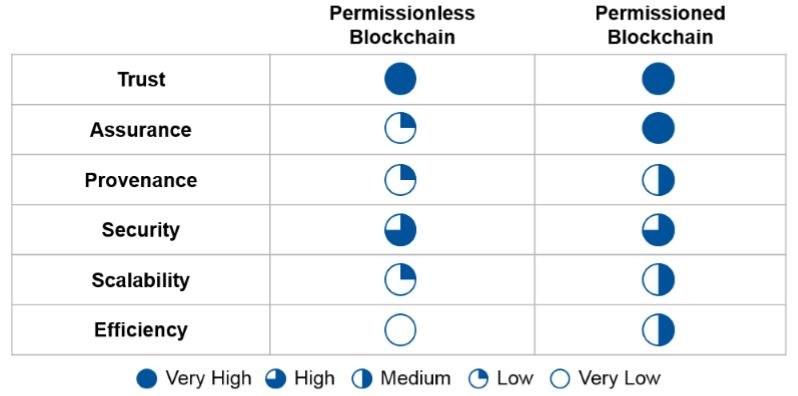
\includegraphics[scale=0.50]{immagini/blockchain_ability_to_implement_ITF}
	\caption{Schema comparativo Permissionless vs Permissioned}
\end{figure} 
\\
Come si può vedere dallo schema la tecnologia migliore da adottare per implementare l'\gls{ITF} è una \textit{permissioned Blockchain}.
I motivi che portano a questa scelta sono:
\begin{itemize}
	\item \textbf{Fiducia (Trust)} - la \textit{permissioned Blockchain} risulta più appropriata per gestire la fiducia ed il rischio in un \gls{ITF} a causa del suo modello di governance che pone un certo controllo su chi può e chi non può accedere alla rete; 
	\item \textbf{Sicurezza (Assurance)} - una \textit{permissionless Blockchain} assicura un livello inferiore di assurance proprio perché permette a qualsiasi nodo, anche uno potenzialmente maligno, di partecipare alla rete cosa che, una \textit{permissioned Blockchain}, non permette;
	\item \textbf{Provenienza (Provenance)} - le \textit{permissionless Blockchain} non condividono un servizio centrale di timing. Le \textit{permissioned Blockchain} riescono, tramite un accordo, ad utilizzare un clock centrale che sincronizza i loro timestamp
	\item \textbf{Scalabilità (Scalability)} - una \textit{permissioned Blockchain} risulta più efficace se sottoposta ad un grande carico di lavoro grazie ai suoi algoritmi di consenso più snelli che non devono garantire la fiducia tra i singoli nodi ma solo che il blocco da inserire, nella \textit{Blockchain}, sia corretto 
	\item \textbf{Efficenza (Efficency)} - conseguenza diretta della Scalabilità e quindi della leggerezza degli algoritmi di consenso, una \textit{permissioned Blockchain} risulta più efficiente, per quanto riguarda i consumi energetici, rispetto alla sua controparte \textit{permissionless}.
\end{itemize}